\subsection{Graph-based Parsing Framework with Latent Alignment}
\label{ssec:graph-based}

\begin{figure*}[h]
\centering
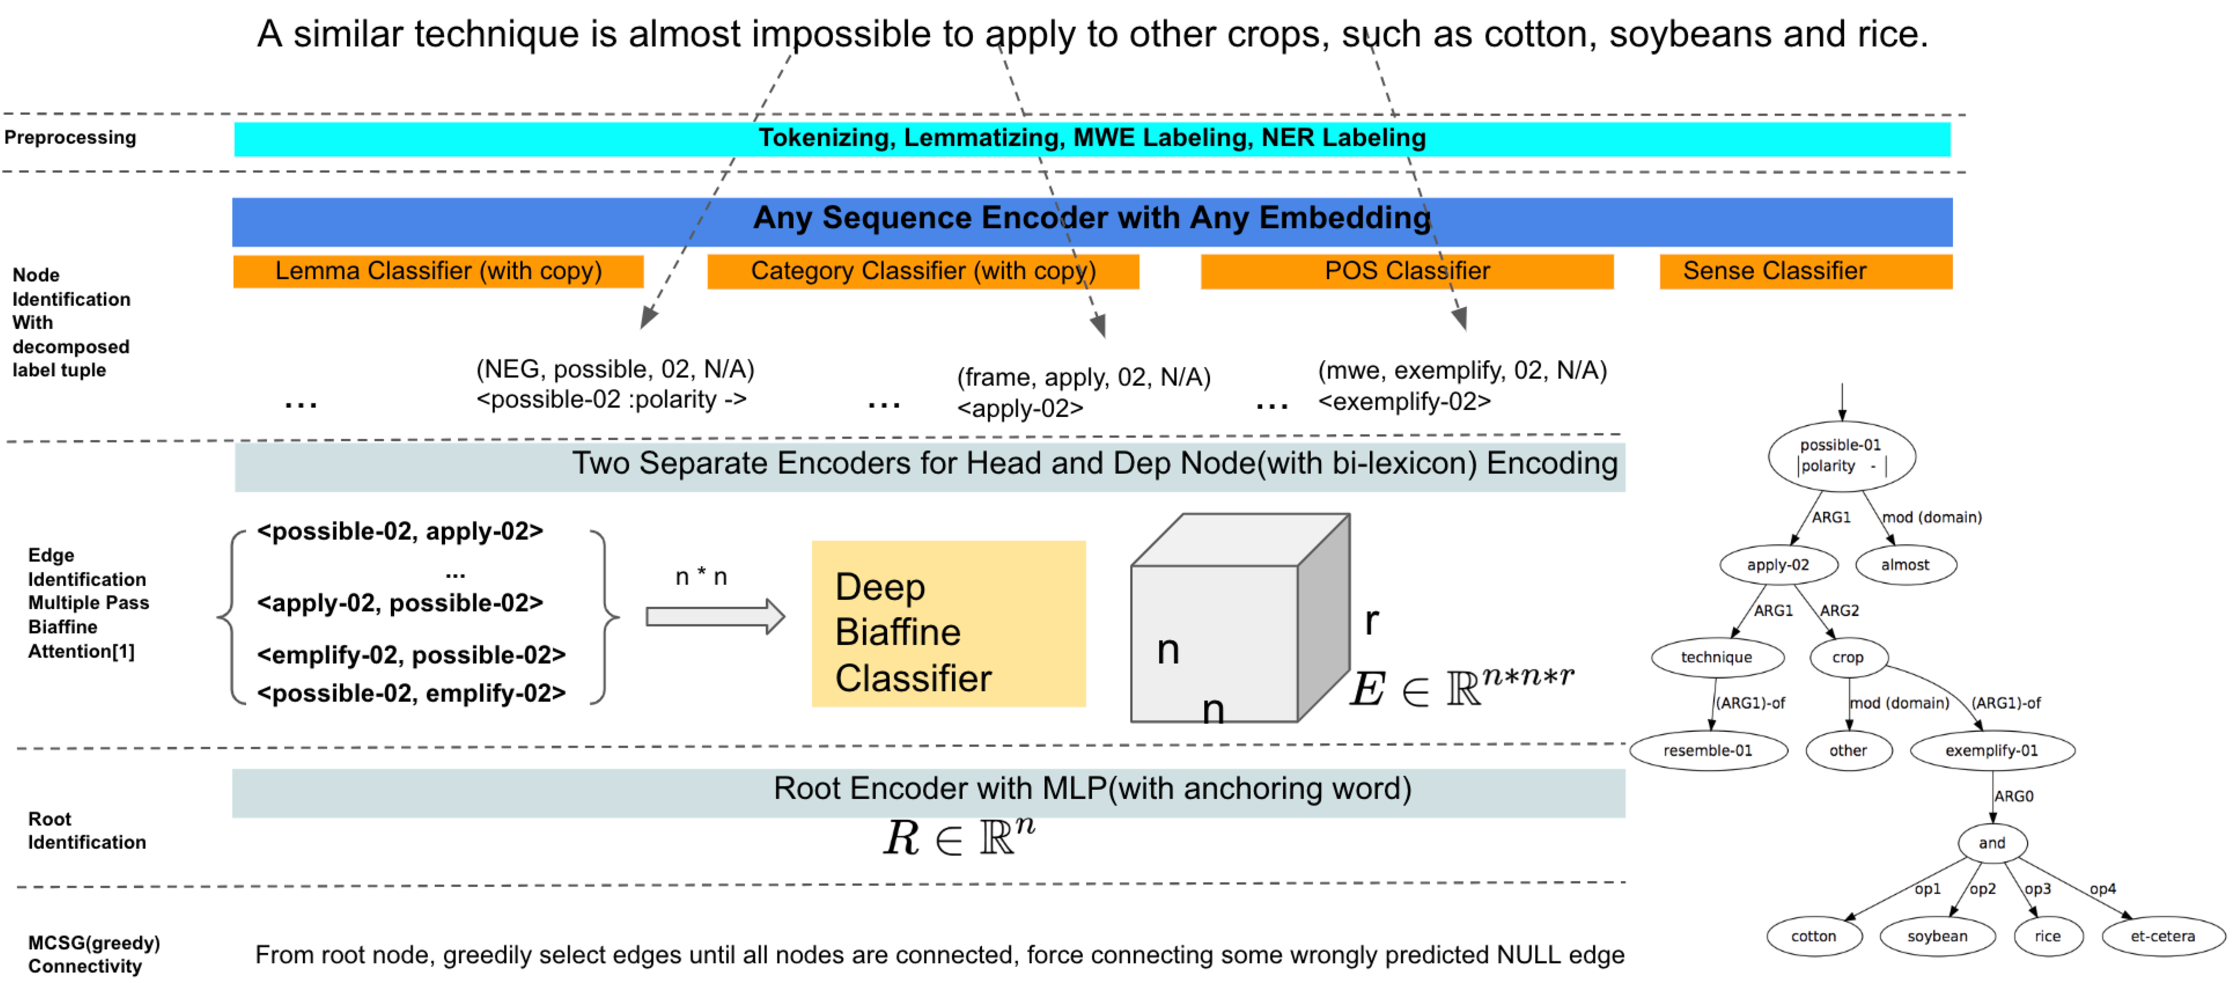
\includegraphics[width=1.00\textwidth]{graph-overview.pdf}
\caption{\label{fig:graph-based-inference} Architecture of graph-based model and inference, for running exmaple [wsj\#0209013]}
\end{figure*}

Before formulating the graph-based model into a probabilistic model as
Equation \ref{eq:graph_prob}, we denote some notations: $C$, $R$ are
sets of concepts (nodes) and relations (edges) in the graph, and $w$
is a sequence of tokens.  $a \in {\mathbb{Z}}^m$ as the alignment
matrix, each $a_{i}$ is the index of aligned token where $i$th node
aligned to. When modeling the negative log likelihood loss~(NLL), with
independence assumption between each node and edge, we decompose it
into node- and edge-identification pipelines.
\begin{equation}
  \label{eq:graph_prob}
\begin{aligned} \smaller[2]
 & NLL(P(C,R \mid w)) \\
 & = - \log(P(C,R \mid w)) \\
 & = - \log(\sum_{a}{P(a) P(C,R \mid w,a)}) \\
 & = - \log\left(\sum_{a}P(a) P(R\mid w,a,c) P(c \mid w, a)\right) \\
 & = - \log\left(\sum_{a}P(a) \prod_{i}^{m} P(c_{i} \mid h_{a_{i}}) \right. \\
 & \qquad \left.\cdot \prod_{i,j=1}^{m}P(r_{ij} \mid h_{a_{i}}, c_{i}, h_{a_{j}}, c_{j})\right)
\end{aligned}
\end{equation}

In DM, PSD, and AMR, every token will only be aligned once.  Hence, we
train a joint model to maximize the above probability for both node
identification $P(c_{i} \mid h_{a_{i}})$ and edge identification
$P(r_{ij} \mid h_{{a_{i}}, c_{i},h_{a_{j}}, c_{j}})$, and we need to
marginalize out the discrete alignment variable $a$.

\subsubsection{Alignment Model}
The above model can support both explicit alignments for DM, PSD, and implicit alignments for AMR.

\subparagraph{Explicit Alignments} For DM, PSD, with explicit
alignments $a*$, we can use $P(a^{*}) = 1.0$ and other
alignments $P(a | a \neq a^{*}) = 0.0 $

\subparagraph{Implicit Alignments} For AMR, without gold alignments,
one requires to compute all the valid alignments and then
condition the node- and edge-identification methods on the alignments.
\begin{equation}
 \label{eq:elbo}
\begin{aligned} \smaller[2]
  & \log(P(C,R \mid w)) \geq \\
  & E_{Q}[\log(P_{\theta}(c\mid w,a) P_{\Phi}(R\mid w,a,c))] \\
  & - \kld{Q_{\Psi}(a\mid c, R,w)}{P(a)}
\end{aligned}
\end{equation}
However, it is computationally intractable to enumerate all
alignments. We estimate posterior alignments model $Q$ as Equation \ref{eq:posterior_prob}, please refer to
\citet{lyu2018amr} for more details.
%\footnote{We fixed an implementation
%  error when computing KL-divergence with implicit Gumbel-Sinkhorn
%  distribution}:

\begin{itemize}
\item Applying variational inference to reduce it into
  Evidence Lower Bound~\cite[ELBO,][]{kingma2013auto}
\item The denominator $Z_{\Psi}$ in Q can be estimated by Perturb-and-Max(MAP)~\cite{papandreouperturb}
\begin{equation}
  \label{eq:posterior_prob}
\begin{aligned} \smaller[2]
Q_{\Psi}(a\mid c, R,w)= \frac{\exp(\sum_{i=1}^{n} \phi(g_{i}, h_{a_{i}}))} {Z_{\Psi}(c,w)}
\end{aligned}
\end{equation}
Where $\phi(g_{i}, h_{a_{i}})$ score each alignment link between node i and the corresponding words,
$g_{i}$ is node encoding, and $h_{a_{i}}$ is encoding for the aligned token.

\item Discrete \texttt{argmax} of a permutation can be estimated by
  Gumbel-Softmax Sinkhorn Networks \cite{mena2018learning, lyu2018amr}
\end{itemize}

\subsubsection{Node Identification}
\label{ssec:node_ident}
Node Identification predicts a concept $c$ given a word. A
concept can be either {\it NULL} (when there is no semantic node
anchoring to that word, e.g., the word is dropped), or a node label
(e.g., lemma, sense, POS, name value in AMR, frame value in PSD), or
other node properties. One challenge in node identification is the
data sparsity issue. Many of the labels are from open sets derived
from the input token, e.g., its lemma.  Moreover, some labels are
constrained by a deterministic label set given the word. Hence, we
designed a copy mechanism~\cite{luong2014addressing} in our neural
network architecture to decide whether to copying deterministic label
given a word or estimate a classification probability from a fixed
label set.


\subsubsection{Edge Identification}
\label{ssec:edge_ident}

By assuming the independence of each edge, we model the edges
probabilites independently.  Given two nodes and their underlying
tokens, we predict the edge label as the semantic relation between the
two concepts with a bi-affine classifier~\cite{dozat2016deep}.

\subsubsection{Inference}
In our two-stage graph-based parsing, after nodes are identified, edge
identification only output a probility distribution over all the
relations between identified nodes. However, we need to an inference
algorithm to search for the maximum spanning connected graph from all
the relations. We use ~\citet[MSCG,][]{Flanigan:2014vc} to greedily
select the most valuable edges from the identified nodes and their
relations connecting them. As shown in Figure
\ref{fig:graph-based-inference}, an input sentence goes through
preprocessing, node identification, edge identification, root
identification, and MCSG to generate a final connected graph as
structured output.

%%% Local Variables:
%%% mode: latex
%%% TeX-master: "main"
%%% End:
